% prerequisite: use inkscape to convert
% arch.svg to arch.tikz
% resulthier.svg to resulthier.tikz
\documentclass{beamer}

\usepackage{graphics}
\usepackage{hyperref}
\usepackage{tikz}

\title{Project LAHTeX}
\author{L.A.H.}

\setbeamertemplate{enumerate item}{(\arabic{enumi})}

\newcommand{\TeXPortal}{\TeX P$\mathcal{O}$rtal}

\begin{document}

\begin{frame}
\titlepage
\begin{center}
\scriptsize{This slide is compiled using \TeXPortal}
\end{center}
\end{frame}

\begin{frame}[fragile]{Introduction}
\verb/LAHTeX/ is a project aiming to provide a simple Java library interface to support management and utilization of TeX Live \TeX\ and \LaTeX\ distribution
\begin{itemize}
\item In particular, it provides back--end service to my \TeXPortal\ Android application
\item Note that the library could be extended to obtain a TeX Live manager on PC as well!
\item This project depends on my \verb/LAHSpectre/ project for process invocation, streams processing and common interfaces.
\end{itemize}
\end{frame}

\begin{frame}[fragile]{Operational architecture}



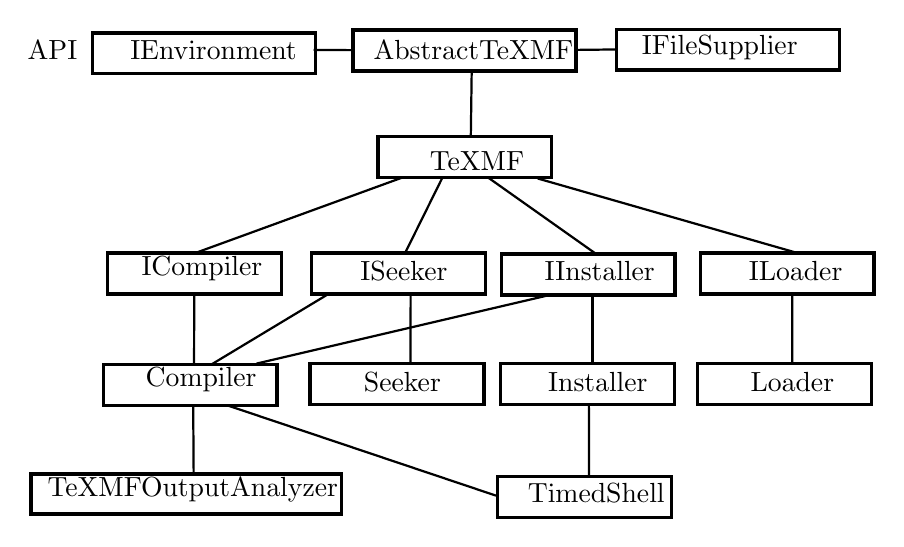
\begin{tikzpicture}[y=0.80pt, x=0.8pt,yscale=-1, inner sep=0pt, outer sep=0pt]
\path[fill=black] (46.335152,102.36218) node[above right] (text2996)
  {IEnvironment};
\path[fill=black] (277.41241,102.36218) node[above right] (text3000)
  {IFileSupplier};
\path[fill=black] (156.23064,102.36218) node[above right] (text3004)
  {AbstractTeXMF};
\path[fill=black] (181.71588,152.36218) node[above right] (text3008) {TeXMF};
\path[fill=black] (51.414215,202.36218) node[above right] (text3012)
  {ICompiler};
\path[fill=black] (233.52258,202.36218) node[above right] (text3016)
  {IInstaller};
\path[fill=black] (325.75415,202.36218) node[above right] (text3020) {ILoader};
\path[fill=black] (150.3179,202.36218) node[above right] (text3024) {ISeeker};
\path[fill=black] (9.0289993,302.36218) node[above right] (text3028)
  {TeXMFOutputAnalyzer};
\path[fill=black] (53.309246,252.36218) node[above right] (text3036) {Compiler};
\path[fill=black] (151.8878,252.36218) node[above right] (text3040) {Seeker};
\path[fill=black] (235.09248,252.36218) node[above right] (text3044)
  {Installer};
\path[fill=black] (326.53909,252.36218) node[above right] (text3048) {Loader};
\path[draw=black,miter limit=4.00,line width=1.350pt,rounded corners=0.0000cm]
  (29.2292,90.4079) rectangle (129.9661,108.7034);
\path[draw=black,miter limit=4.00,line width=1.350pt,rounded corners=0.0000cm]
  (265.9772,88.8711) rectangle (366.7141,107.1666);
\path[draw=black,miter limit=4.00,line width=1.350pt,rounded corners=0.0000cm]
  (147.0607,89.2229) rectangle (247.7976,107.5183);
\path[draw=black,miter limit=4.00,line width=1.199pt,rounded corners=0.0000cm]
  (158.1641,137.2792) rectangle (236.6657,155.7809);
\path[draw=black,miter limit=4.00,line width=1.199pt,rounded corners=0.0000cm]
  (36.1044,189.8709) rectangle (114.6060,208.3725);
\path[draw=black,miter limit=4.00,line width=1.199pt,rounded corners=0.0000cm]
  (128.3360,189.8709) rectangle (206.8376,208.3725);
\path[draw=black,miter limit=4.00,line width=1.199pt,rounded corners=0.0000cm]
  (213.8955,190.2634) rectangle (292.3972,208.7650);
\path[draw=black,miter limit=4.00,line width=1.199pt,rounded corners=0.0000cm]
  (303.7722,189.8709) rectangle (382.2739,208.3725);
\path[draw=black,miter limit=4.00,line width=1.199pt,rounded corners=0.0000cm]
  (34.1420,240.1077) rectangle (112.6436,258.6093);
\path[draw=black,miter limit=4.00,line width=1.199pt,rounded corners=0.0000cm]
  (127.5510,239.7152) rectangle (206.0527,258.2168);
\path[draw=black,miter limit=4.00,line width=1.199pt,rounded corners=0.0000cm]
  (213.5030,239.7152) rectangle (292.0047,258.2168);
\path[draw=black,miter limit=4.00,line width=1.199pt,rounded corners=0.0000cm]
  (302.5948,239.7152) rectangle (381.0965,258.2168);
\path[draw=black,miter limit=4.00,line width=1.200pt,rounded corners=0.0000cm]
  (1.5714,289.6916) rectangle (141.7577,307.6992);
\path[fill=black] (225.90265,302.36218) node[above right] (text3917)
  {TimedShell};
\path[draw=black,miter limit=4.00,line width=1.199pt,rounded corners=0.0000cm]
  (212.1838,290.7501) rectangle (290.6855,309.2517);
\path[draw=black,line join=miter,line cap=butt,line width=0.800pt]
  (200.1622,136.8668) -- (200.5547,107.8713);
\path[draw=black,line join=miter,line cap=butt,line width=0.800pt]
  (248.2159,98.0594) -- (265.9018,97.8632);
\path[draw=black,line join=miter,line cap=butt,line width=0.800pt]
  (146.3650,98.1744) -- (129.1242,98.0594);
\path[draw=black,line join=miter,line cap=butt,line width=0.800pt]
  (169.4934,155.6243) -- (76.5326,189.5061);
\path[draw=black,line join=miter,line cap=butt,line width=0.800pt]
  (187.2779,155.8682) -- (170.3341,190.0948);
\path[draw=black,line join=miter,line cap=butt,line width=0.800pt]
  (208.0117,155.7532) -- (256.2861,189.8985);
\path[draw=black,line join=miter,line cap=butt,line width=0.800pt]
  (230.3828,156.1457) -- (348.7140,190.0948);
\path[draw=black,line join=miter,line cap=butt,line width=0.800pt]
  (75.1589,239.9391) -- (75.2263,207.5123);
\path[draw=black,line join=miter,line cap=butt,line width=0.800pt]
  (172.8852,240.1353) -- (172.9804,208.5074);
\path[draw=black,line join=miter,line cap=butt,line width=0.800pt]
  (255.1087,239.7429) -- (255.1087,208.9336);
\path[draw=black,line join=miter,line cap=butt,line width=0.800pt]
  (345.3779,239.7429) -- (345.3541,208.8761);
\path[draw=black,line join=miter,line cap=butt,line width=0.800pt]
  (74.7665,258.9741) -- (74.9627,289.3909);
\path[draw=black,line join=miter,line cap=butt,line width=0.800pt]
  (90.0730,258.5817) -- (211.5440,299.3990);
\path[draw=black,line join=miter,line cap=butt,line width=0.800pt]
  (253.4897,258.8760) -- (253.5389,290.2740);
\path[fill=black] (0,102.36218) node[above right] (text3121) {API};
\path[draw=black,line join=miter,line cap=butt,line width=0.800pt]
  (83.0084,240.1353) -- (135.7963,208.3449);
\path[draw=black,line join=miter,line cap=butt,line width=0.800pt]
  (103.4171,239.7429) -- (235.0925,208.9336);

\end{tikzpicture}


\end{frame}

\begin{frame}[fragile]{Main API}
Defined at the top level and third level
\begin{itemize}
\item Client obtains an instance of abstract class \verb/AbstractTeXMF/ via the static method \verb/getInstance(env)/ where \verb/env/ implements the \verb/IEnvironment/ interface that provides distribution specific information such as system architecture, location to store binaries and \TeX\ directories, etc.
\item \verb/AbstractTeXMF/ combines services defined by \verb/IInstaller/, \verb/ICompiler/, etc interfaces namely compile a document \& analyzes the output for missing packages, install a package, search for a package providing a file, retrieve the list of available packages.
\end{itemize}
\textbf{Implementation}: \verb/TeXMF/ implements \verb/AbstractTeXMF/ simply by delegating requests to specific operators.
\end{frame}

\begin{frame}[fragile]{Result hierarchy}
API methods return an instance of \verb/IResult/ which contains any (first) \verb/Exception/ raised in its execution. The result hierarchy:\\\vspace{0.25cm}
\scalebox{0.7}{



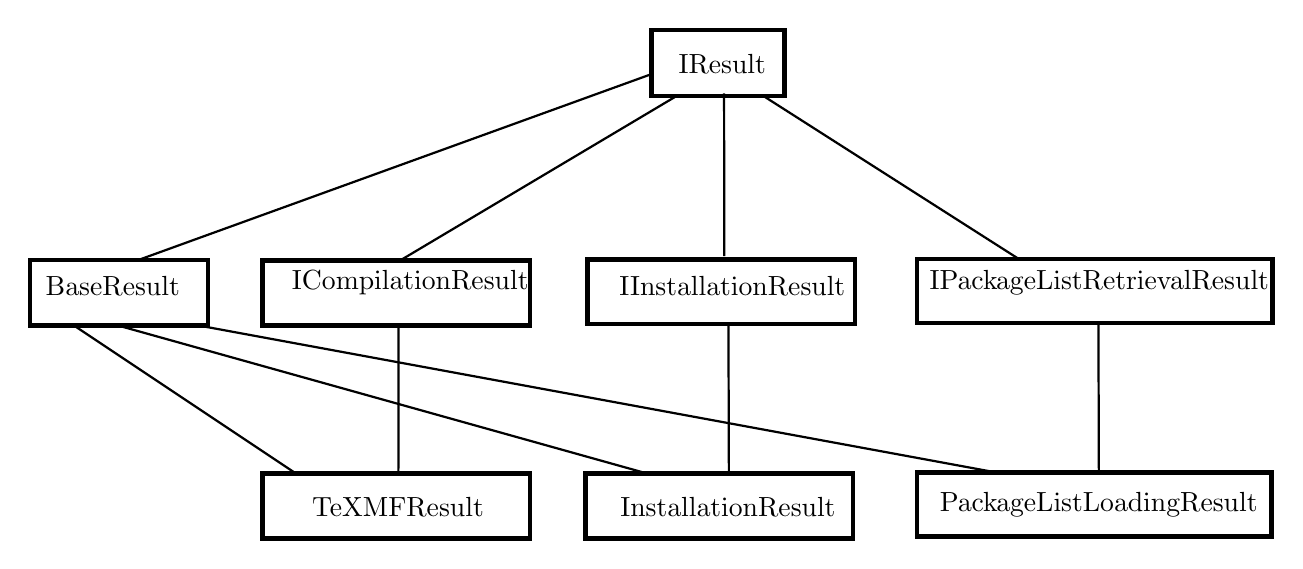
\begin{tikzpicture}[y=0.80pt, x=0.8pt,yscale=-1, inner sep=0pt, outer sep=0pt]
\path[fill=black] (301.56244,152.36218) node[above right] (text3007) {IResult};
\path[fill=black] (126.96598,252.36218) node[above right] (text3011)
  {ICompilationResult};
\path[fill=black] (274.81775,252.36218) node[above right] (text3015)
  {IInstallationResult};
\path[fill=black] (414.96057,252.36218) node[above right] (text3019)
  {IPackageListRetrievalResult};
\path[fill=black] (136.08846,352.36218) node[above right] (text3023)
  {TeXMFResult};
\path[fill=black] (275.27274,352.36218) node[above right] (text3027)
  {InstallationResult};
\path[fill=black] (419.54877,352.36218) node[above right] (text3031)
  {PackageListLoadingResult};
\path[fill=black] (15.74033,252.36218) node[above right] (text3035)
  {BaseResult};
\path[draw=black,miter limit=4.00,line width=1.600pt,rounded corners=0.0000cm]
  (289.2752,132.5647) rectangle (349.4119,162.4396);
\path[draw=black,miter limit=4.00,line width=1.600pt,rounded corners=0.0000cm]
  (8.5776,236.6084) rectangle (88.9509,266.1621);
\path[draw=black,miter limit=4.00,line width=1.600pt,rounded corners=0.0000cm]
  (113.6334,236.7729) rectangle (234.5790,265.9974);
\path[draw=black,miter limit=4.00,line width=1.600pt,rounded corners=0.0000cm]
  (260.4279,236.2141) rectangle (381.3560,265.4417);
\path[draw=black,miter limit=4.00,line width=1.645pt,rounded corners=0.0000cm]
  (409.2054,236.0468) rectangle (569.7263,264.9558);
\path[draw=black,miter limit=4.00,line width=1.600pt,rounded corners=0.0000cm]
  (113.6334,332.9714) rectangle (234.5790,362.1960);
\path[draw=black,miter limit=4.00,line width=1.600pt,rounded corners=0.0000cm]
  (259.4644,332.9699) rectangle (380.3925,362.1975);
\path[draw=black,miter limit=4.00,line width=1.643pt,rounded corners=0.0000cm]
  (409.2070,332.5703) rectangle (569.2667,361.4824);
\path[draw=black,line join=miter,line cap=butt,line width=0.800pt]
  (175.5130,236.8908) -- (300.0606,162.7928);
\path[draw=black,line join=miter,line cap=butt,line width=0.800pt]
  (322.2239,234.7568) -- (322.1324,161.2163);
\path[draw=black,line join=miter,line cap=butt,line width=0.800pt]
  (455.3510,236.1025) -- (339.8686,162.3987);
\path[draw=black,line join=miter,line cap=butt,line width=0.800pt]
  (56.4834,236.8908) -- (289.8130,152.3622);
\path[draw=black,line join=miter,line cap=butt,line width=0.800pt]
  (175.0204,333.1590) -- (175.1189,266.4511);
\path[draw=black,line join=miter,line cap=butt,line width=0.800pt]
  (324.3001,332.3707) -- (324.1031,264.8746);
\path[draw=black,line join=miter,line cap=butt,line width=0.800pt]
  (491.4146,332.1736) -- (491.2175,264.4804);
\path[draw=black,line join=miter,line cap=butt,line width=0.800pt]
  (127.6435,332.2075) -- (28.9846,266.4349);
\path[draw=black,line join=miter,line cap=butt,line width=0.800pt]
  (288.7307,333.3223) -- (49.6082,266.4349);
\path[draw=black,line join=miter,line cap=butt,line width=0.800pt]
  (443.6866,332.2075) -- (86.6890,266.4349);

\end{tikzpicture}


}\\
\vspace{0.25cm}
\textbf{Note}: Instances of \verb/IResult/ are \emph{progressively} built. For example, the log is appended in  \verb/ICompilationResult/ by \verb/ICompiler/ until invocation of \verb/isComplete()/ returns \textbf{true}.
\end{frame}

\begin{frame}[fragile]{Exceptions}
\verb/LAHTeX/ defines 3 \verb/Exception/s classes, all is traced back to some required file being unavailable
\begin{itemize}
\item \verb/KpathseaException/: raised when a \TeX\ format, TeX Font Metric (TFM) file, MetaFont source, Packed Bitmap (PK) font, ... is unavailable

These files are either supplied in some TeX Live package or should be generated using some command (for example, \verb/initex/ to generate format).
\item \verb/SystemFileNotFoundException/: raised when a \verb/LAHTeX/ dependency such as \verb/xz/, \verb/tar/, \verb/ls/, ... executable or file--package \verb/index/ (needed to identify missing package) is missing
\item \verb/TeXMFFileNotFoundException/: raised when \verb/tex/, \verb/pdftex/ or \verb/mf/ cannot find an input file (such as \LaTeX\ styles \verb/*.sty/)
\end{itemize}
\end{frame}

\begin{frame}[fragile]{Implementation details}
\begin{itemize}
\item \textbf{Install a package}: simply compute dependency (using a pre--built \verb/depend/ file) get \& extract the package \& relocate extracted files in the directory structure, regenerate \verb/ls-R/ and do \verb/chmod/; requires
\begin{itemize}
\item An implementation of a system--specific \verb/IFileSupplier/

For instance, \TeXPortal\ obtains files from Dropbox (default) or user--defined mirror using \verb/DownloadManager/ in Android API
\item Standard UNIX programs (namely \verb/tar/, \verb/xz/, \verb/cp/, \verb/rm/, \verb/ls/, \verb/chmod/)

(These programs, except for \verb/xz/, are provided by \verb/busybox/ in \TeXPortal.)
\end{itemize}
\item \textbf{List installed packages}: by listing package description files in the directory \verb_/tlpkg/tlpobj/_
\end{itemize}
\end{frame}

\begin{frame}[fragile]{Implementation details (continued)}
\begin{itemize}
\item \textbf{Package search}: using a pre--built \verb/index/ file in which each line is of form \textbf{package-name/file-list/} where \textbf{file-list} contains all files provided in that package, separated by slash
\item \textbf{Compile documents}: run the process using \verb/TimedShell/, recognize missing file from the standard output $\Rightarrow$ find package(s) provide that missing file
\end{itemize}
\end{frame}

\end{document}